\documentclass[aspectratio=1610]{beamer}
\setbeamertemplate{bibliography item}{\insertbiblabel}
\usefonttheme{professionalfonts}
\usetheme{metropolis}
\usepackage{polyglossia}
\setmainlanguage{german}
\usepackage{amsmath}
\usepackage{amssymb}
\usepackage{mathtools}
\usepackage{graphicx}
\usepackage[version=4]{mhchem}
\usepackage[
  math-style=ISO,
  bold-style=ISO,
  sans-style=italic,
  nabla=upright,
]{unicode-math}
\setmathfont{Latin Modern Math}
\usepackage{blindtext}
\usepackage{fontspec}
\title{Der Weg zur grünen Wiese}
\date{\today}
\author{Steven Becker}
\usepackage{siunitx}
\AtBeginDocument{
\sisetup{
math-rm=\mathrm,
math-micro=μ,
}
}
\usepackage{framed}
\usepackage{biblatex}
\addbibresource{lit.bib}
\usepackage{booktabs}

\begin{document}

\frame{\maketitle}


%\begin{frame}
%\tableofcontents
%\end{frame}


\begin{frame}{ $IV$ curve: $0$ to $\SI{130}{\volt}$}

  \begin{columns}

   \begin{column}{0.48\textwidth}
     \begin{figure}
       \centering
       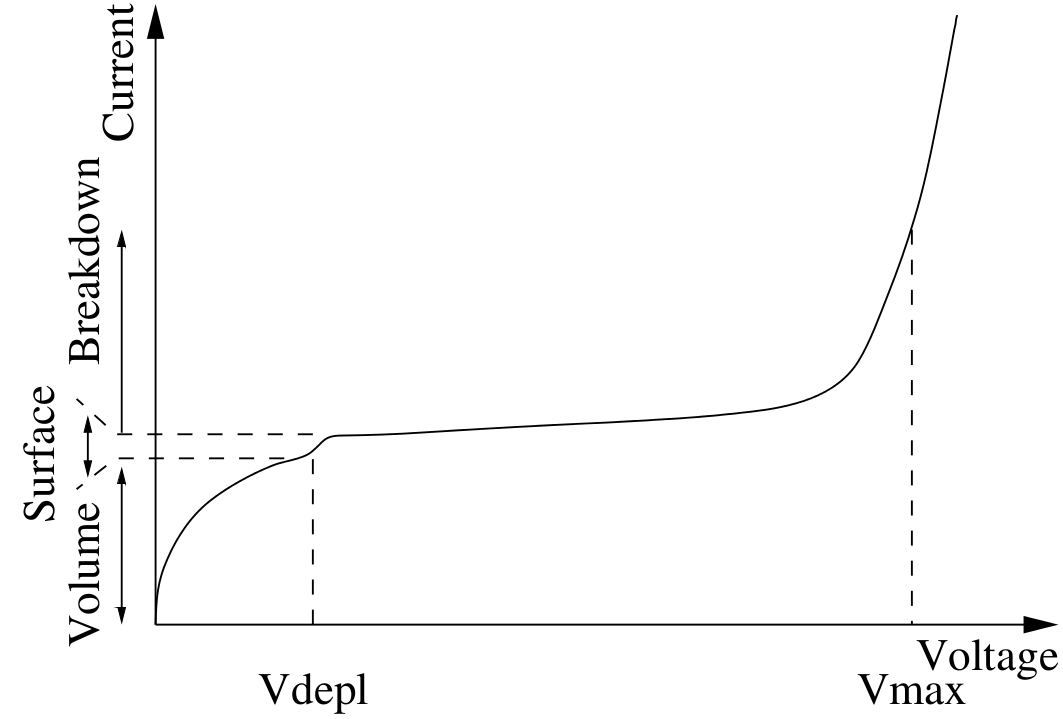
\includegraphics[width=1.05\textwidth]{./iv_curve_reverse_bias_pixel_detectors.png}
       \caption{ Theoretical $IV$ curve \cite{pixel_detectors}. }
       \label{ fig: iv_curve_theoretical}
     \end{figure}
   \end{column}

   \begin{column}{0.48\textwidth}
     \begin{figure}
       \centering
       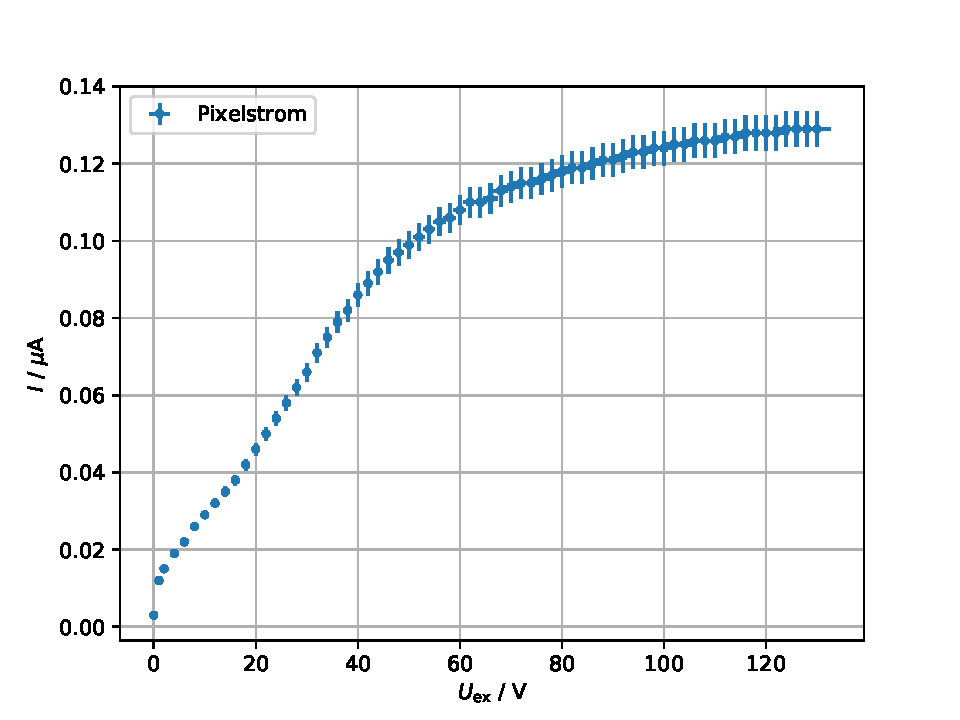
\includegraphics[width=1.05\textwidth]{./iv_curve_0_130_V.pdf}
       \caption{Measured $IV$ curve. }
       \label{ fig: iv_curve_measured}
     \end{figure}
   \end{column}

  \end{columns}

\end{frame}

\section{Laserwidth}

\begin{frame}{ Measurment - $\SI{5}{\milli\meter}$ }

  \begin{figure}
    \centering
    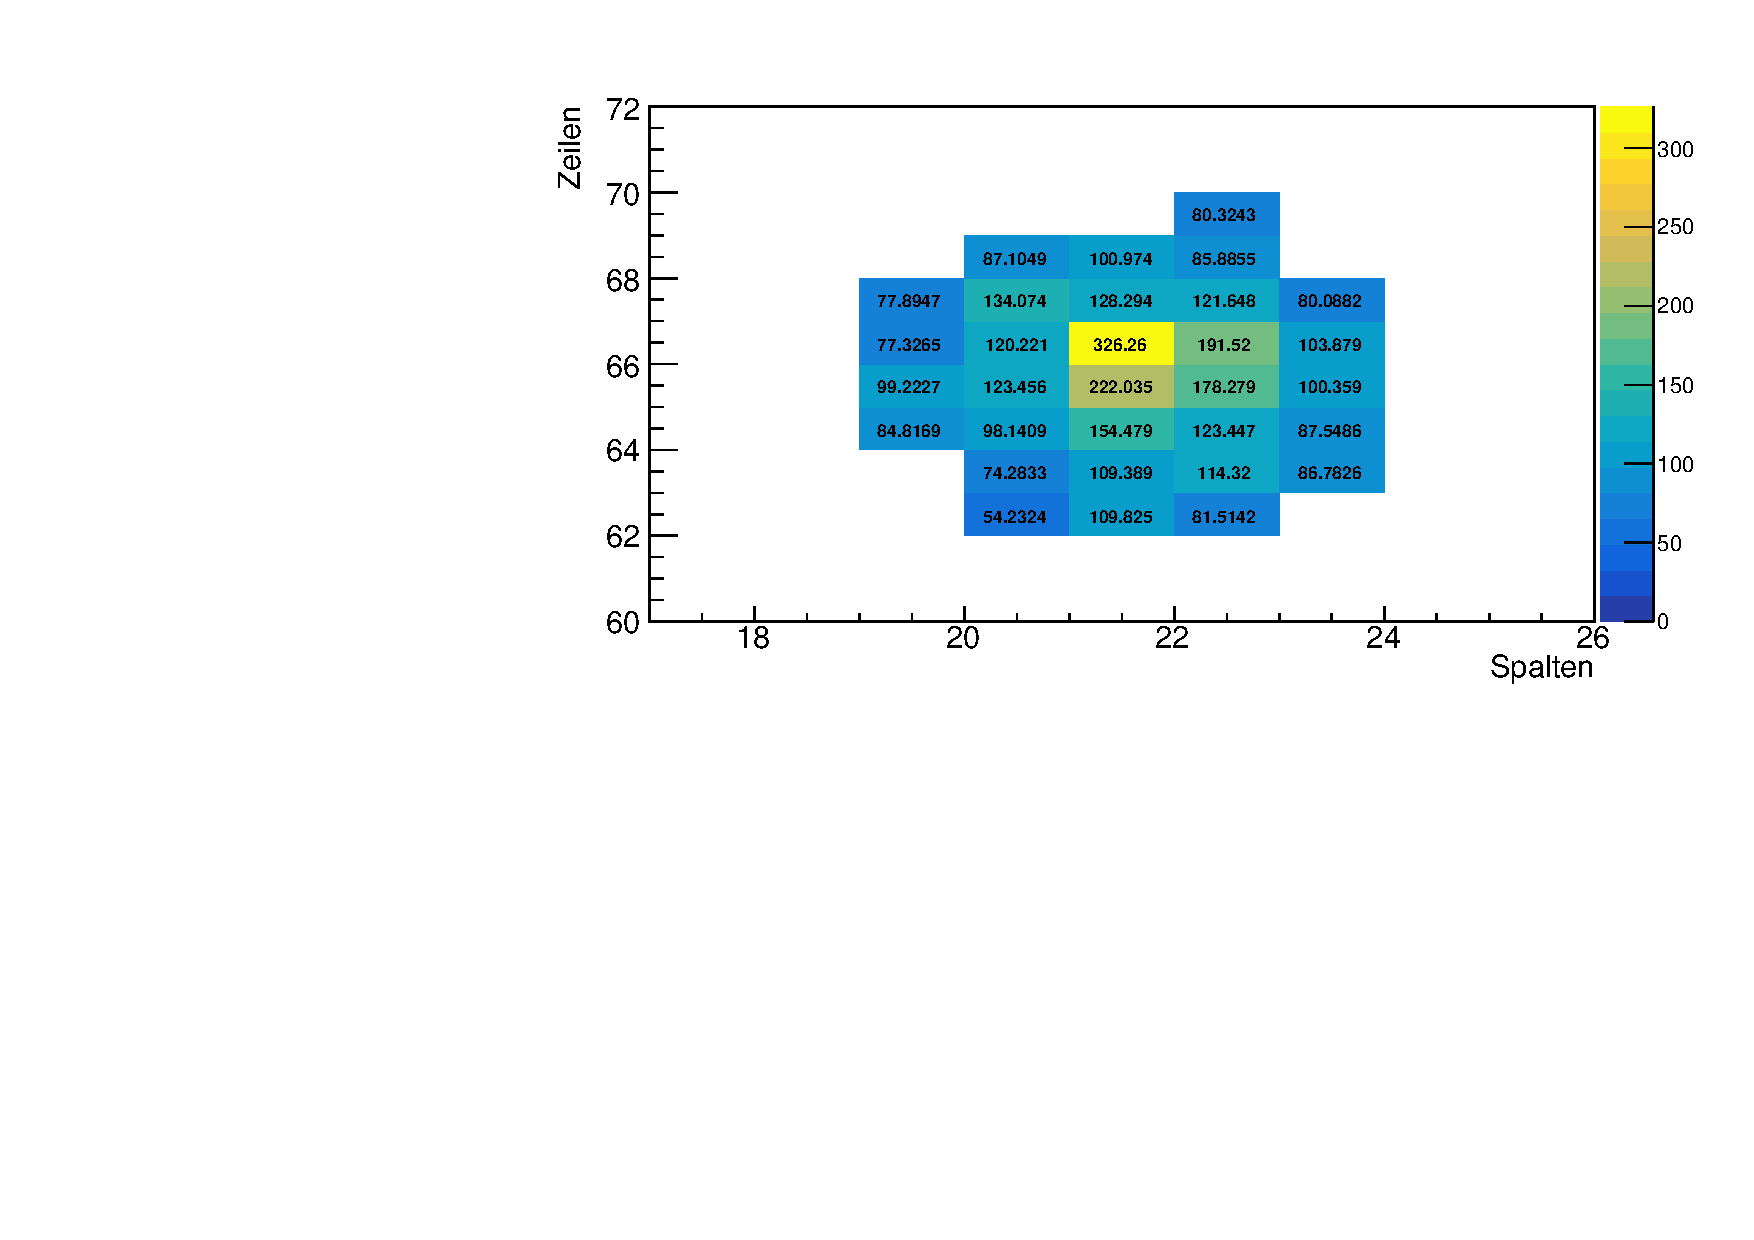
\includegraphics[width=\textwidth]{./5_mm_measurment_plot.pdf}
    \caption{Measured Laserbeam }
    \label{ fig: 5_mm }
  \end{figure}

\end{frame}


\begin{frame}{ Fit - $\SI{5}{\milli\meter}$ }
  \begin{columns}

   \begin{column}{0.48\textwidth}
     \begin{figure}
       \centering
       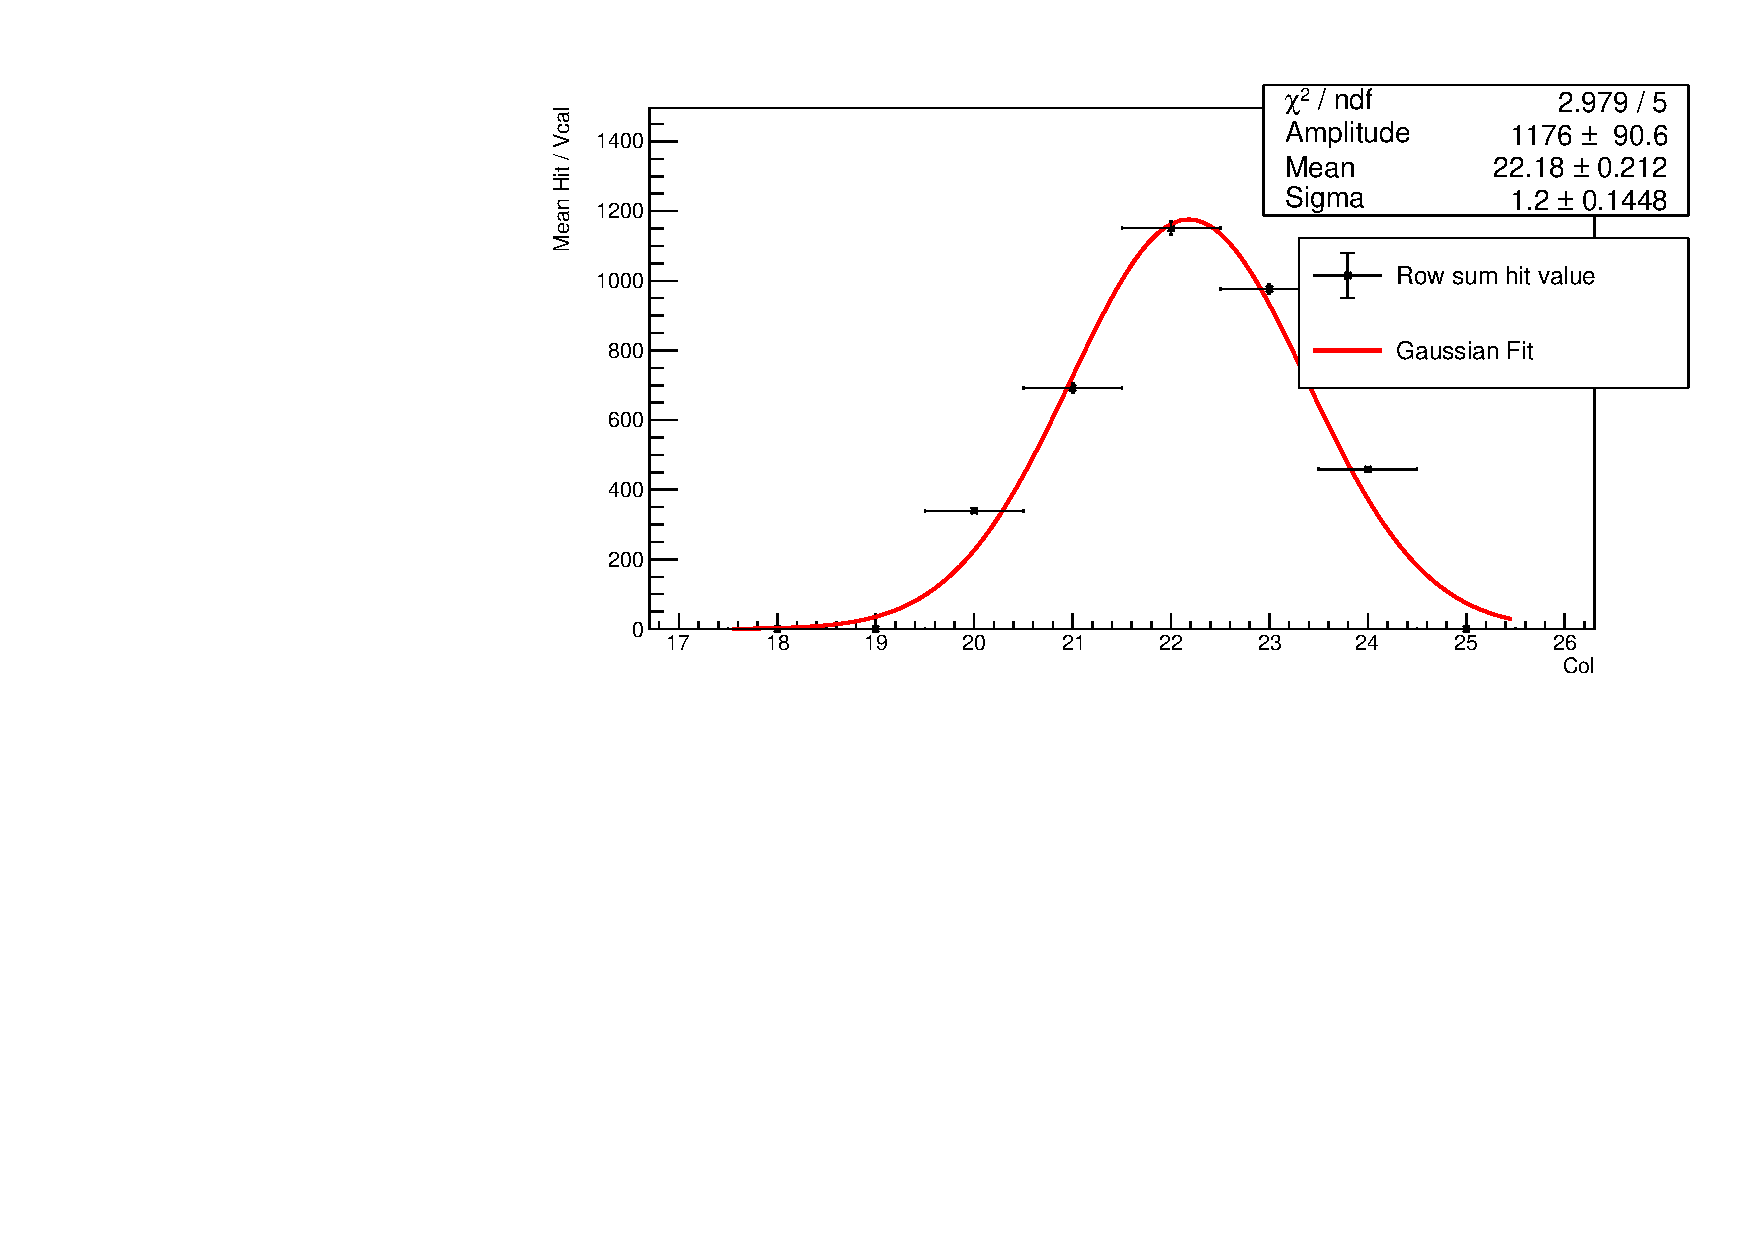
\includegraphics[width=1.05\textwidth]{./5_mm_erorbar_plot_col.pdf}
       \caption{ Fit Columns }
       \label{ fig: iv_curve_theoretical}
     \end{figure}
   \end{column}

   \begin{column}{0.48\textwidth}
     \begin{figure}
       \centering
       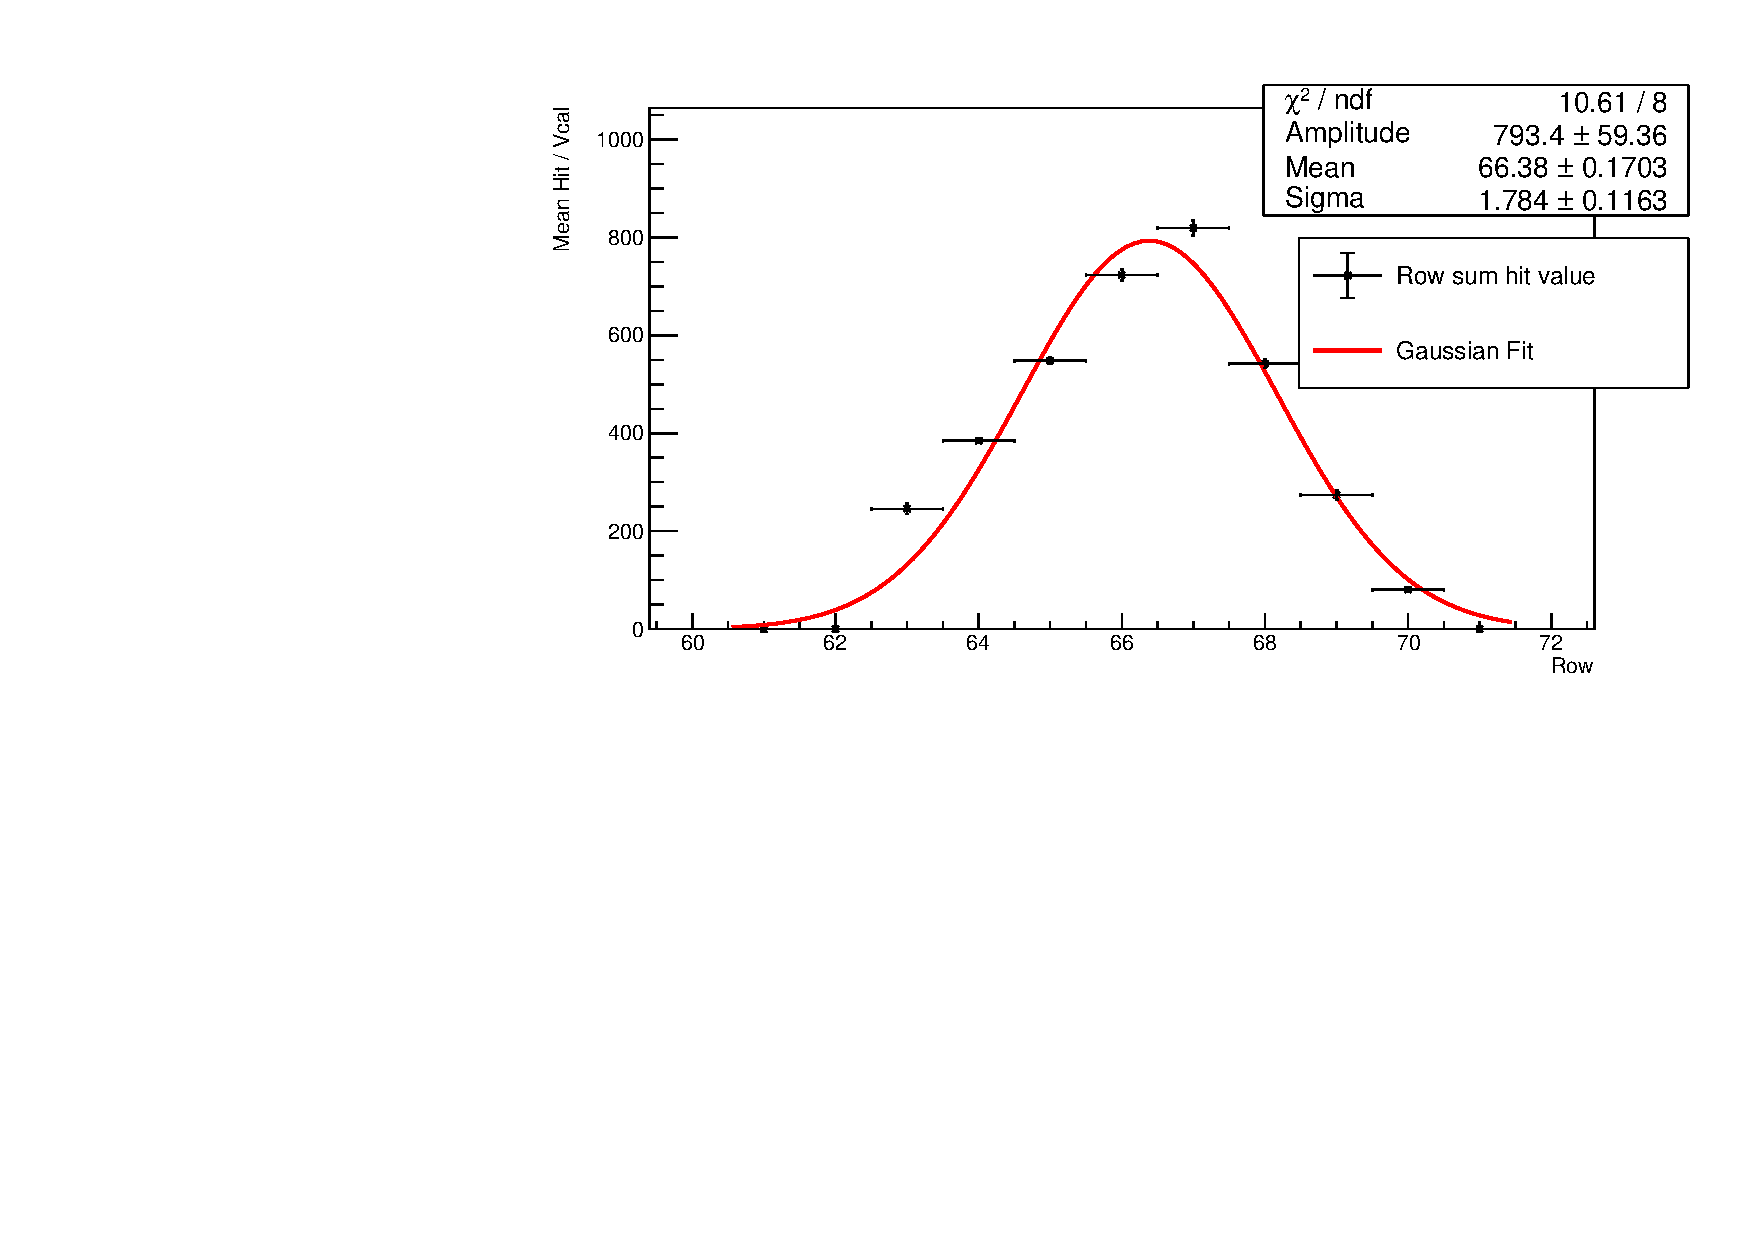
\includegraphics[width=1.05\textwidth]{./5_mm_erorbar_plot_row.pdf}
       \caption{ Fit Rows }
       \label{ fig: iv_curve_measured}
     \end{figure}
   \end{column}

  \end{columns}

\end{frame}

\begin{frame}{ Measurment - $\SI{9}{\milli\meter}$ }

  \begin{figure}
    \centering
    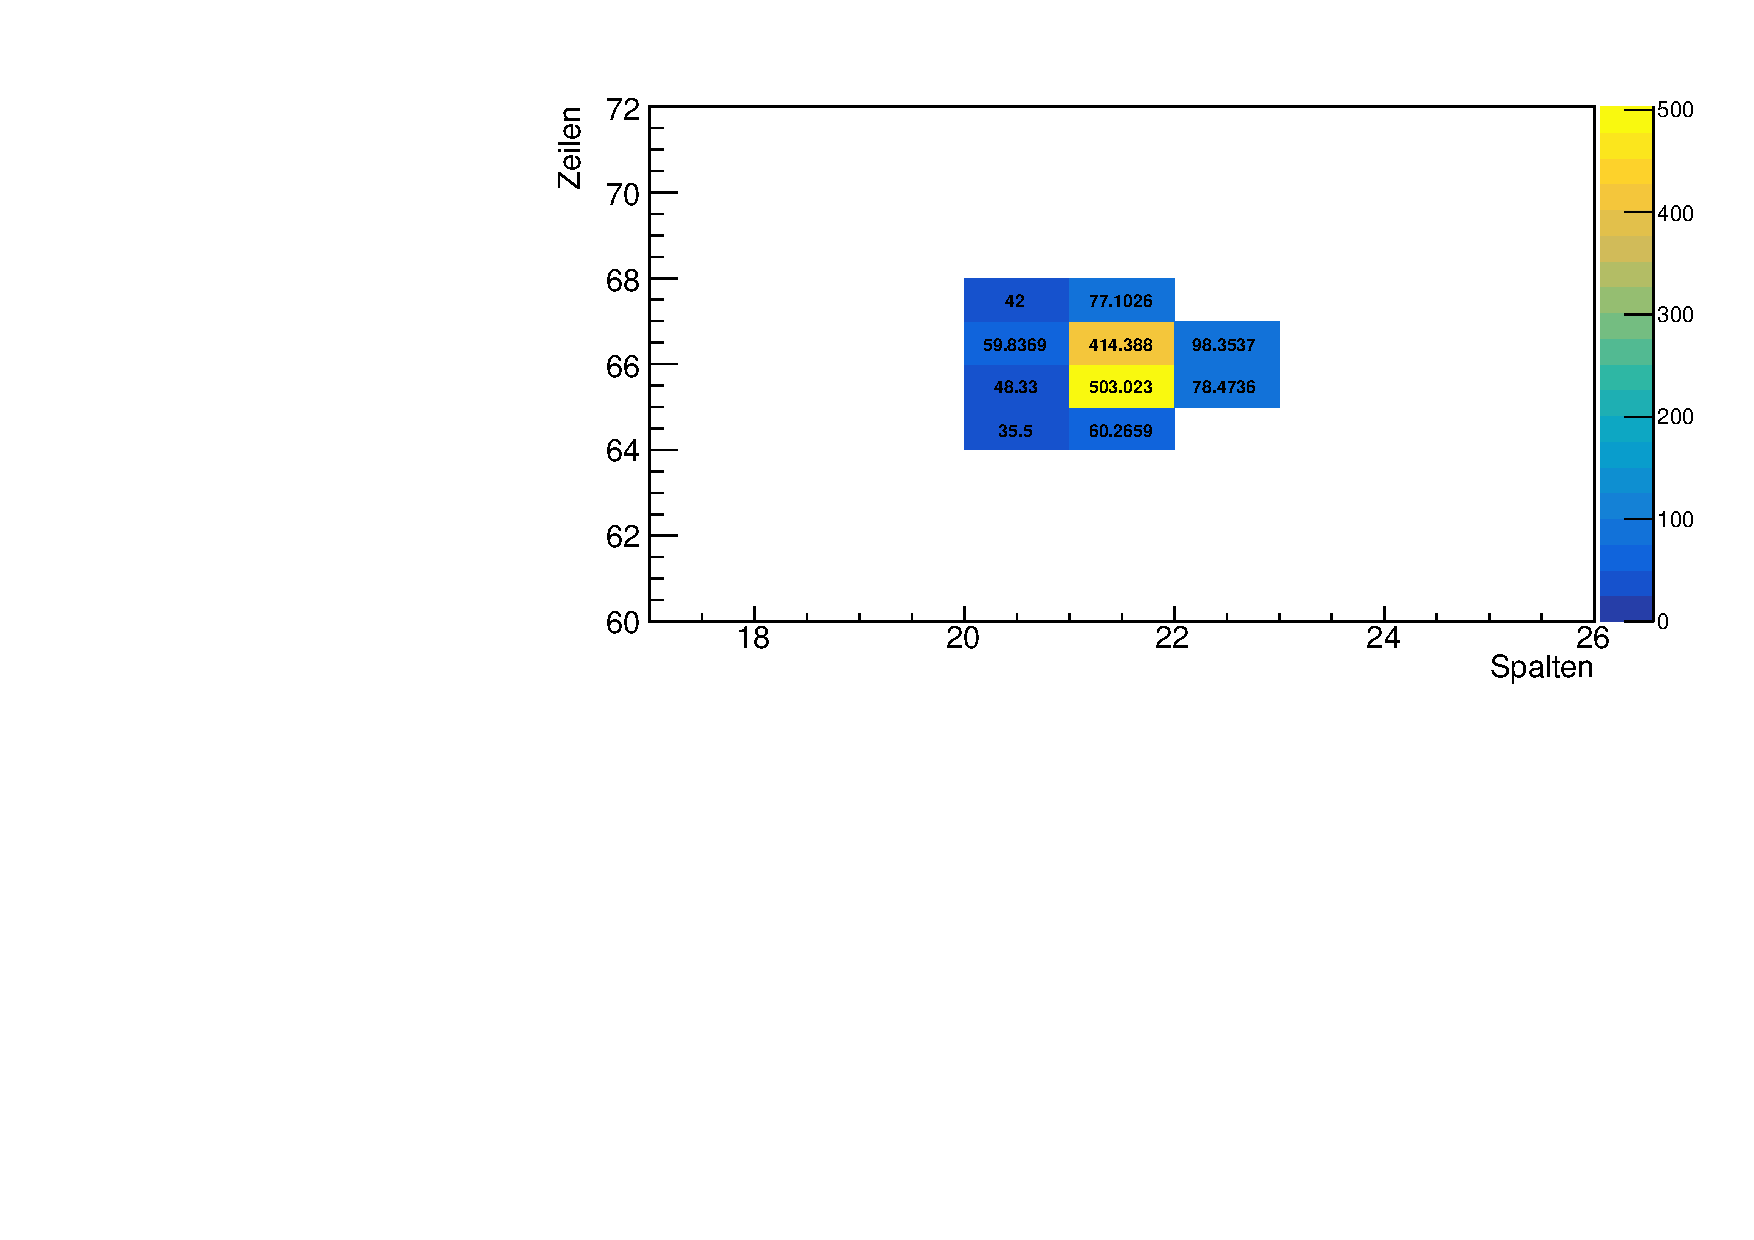
\includegraphics[width=\textwidth]{./9_mm_measurment_plot.pdf}
    \caption{Measured Laserbeam }
    \label{ fig: 5_mm }
  \end{figure}

\end{frame}


\begin{frame}{ Fit - $\SI{9}{\milli\meter}$ }
  \begin{columns}

   \begin{column}{0.48\textwidth}
     \begin{figure}
       \centering
       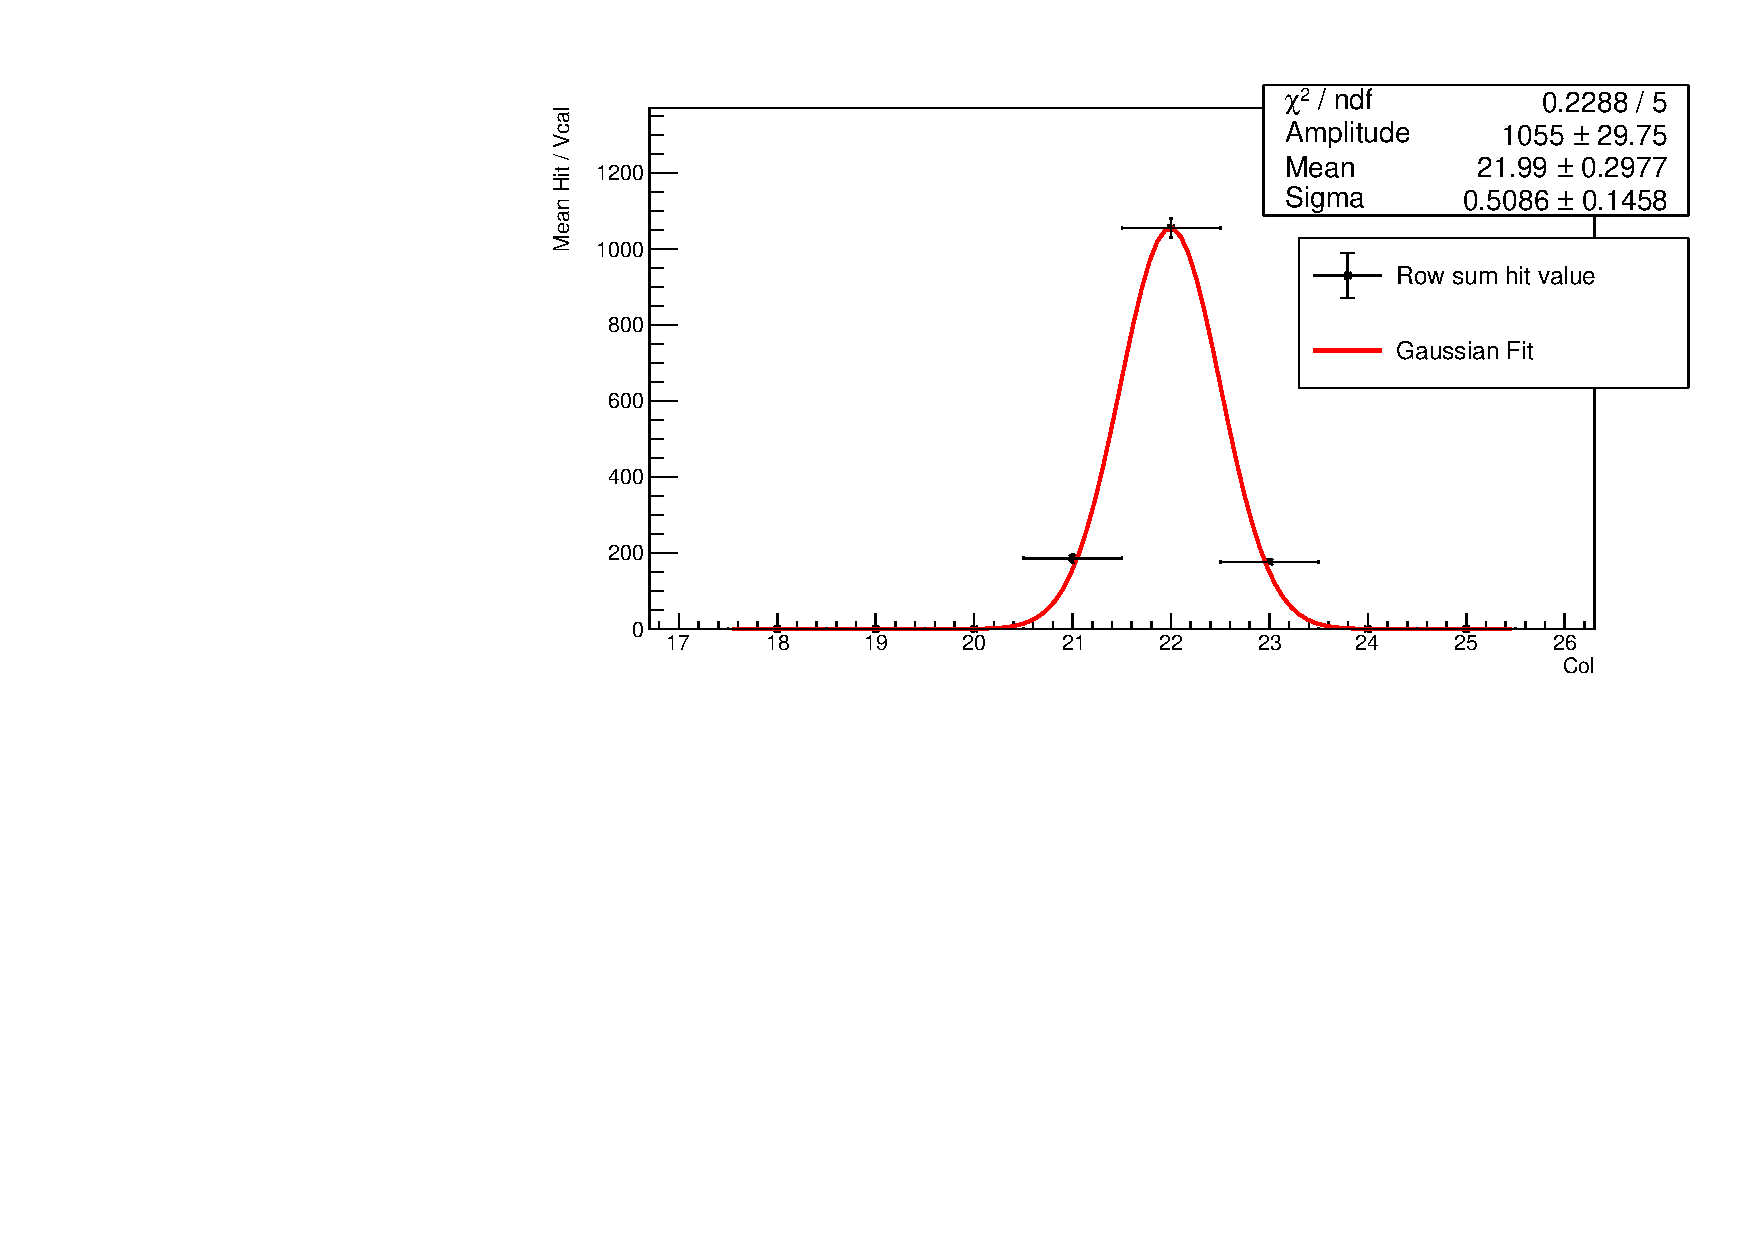
\includegraphics[width=1.05\textwidth]{./9_mm_erorbar_plot_col.pdf}
       \caption{ Fit Columns }
       \label{ fig: iv_curve_theoretical}
     \end{figure}
   \end{column}

   \begin{column}{0.48\textwidth}
     \begin{figure}
       \centering
       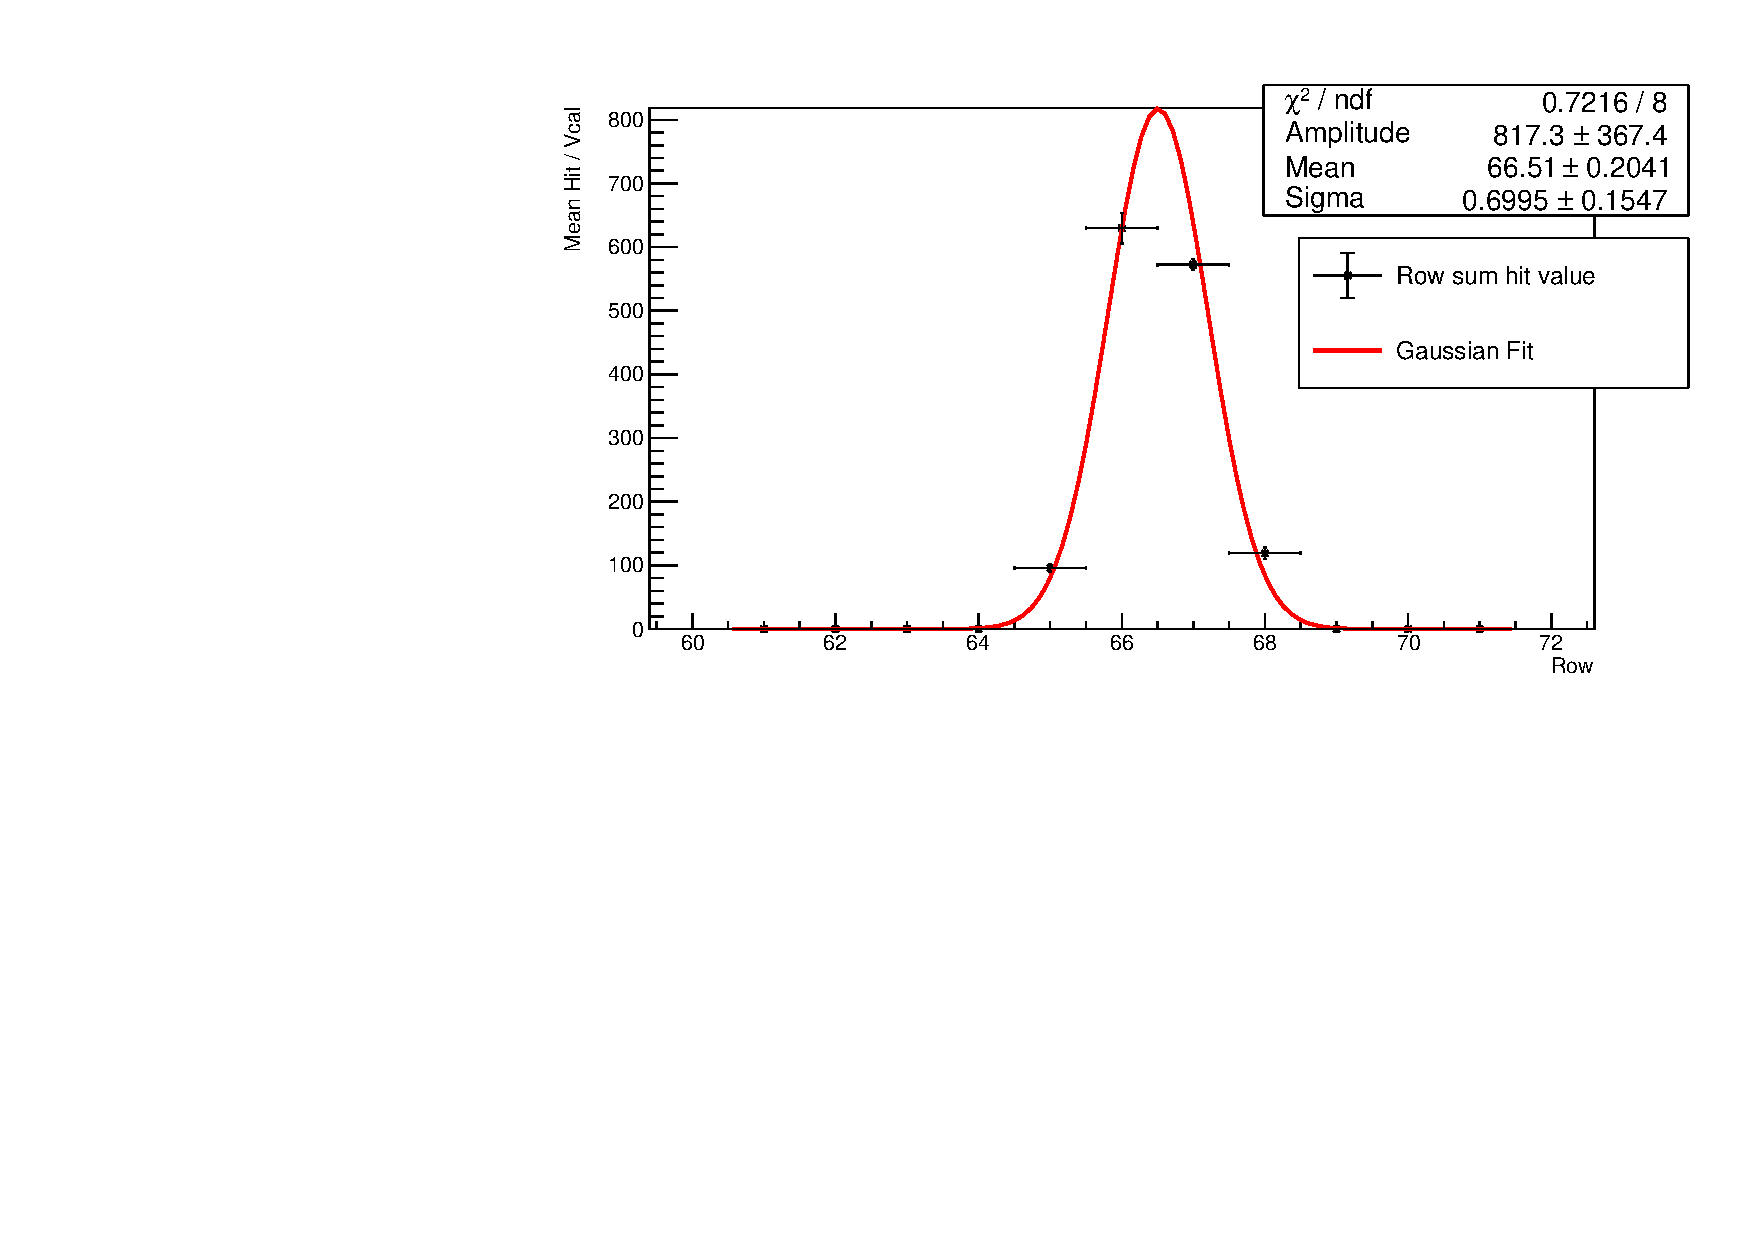
\includegraphics[width=1.05\textwidth]{./9_mm_erorbar_plot_row.pdf}
       \caption{ Fit Rows }
       \label{ fig: iv_curve_measured}
     \end{figure}
   \end{column}

  \end{columns}

\end{frame}


\begin{frame}{ Measurment - $\SI{15}{\milli\meter}$ }

  \begin{figure}
    \centering
    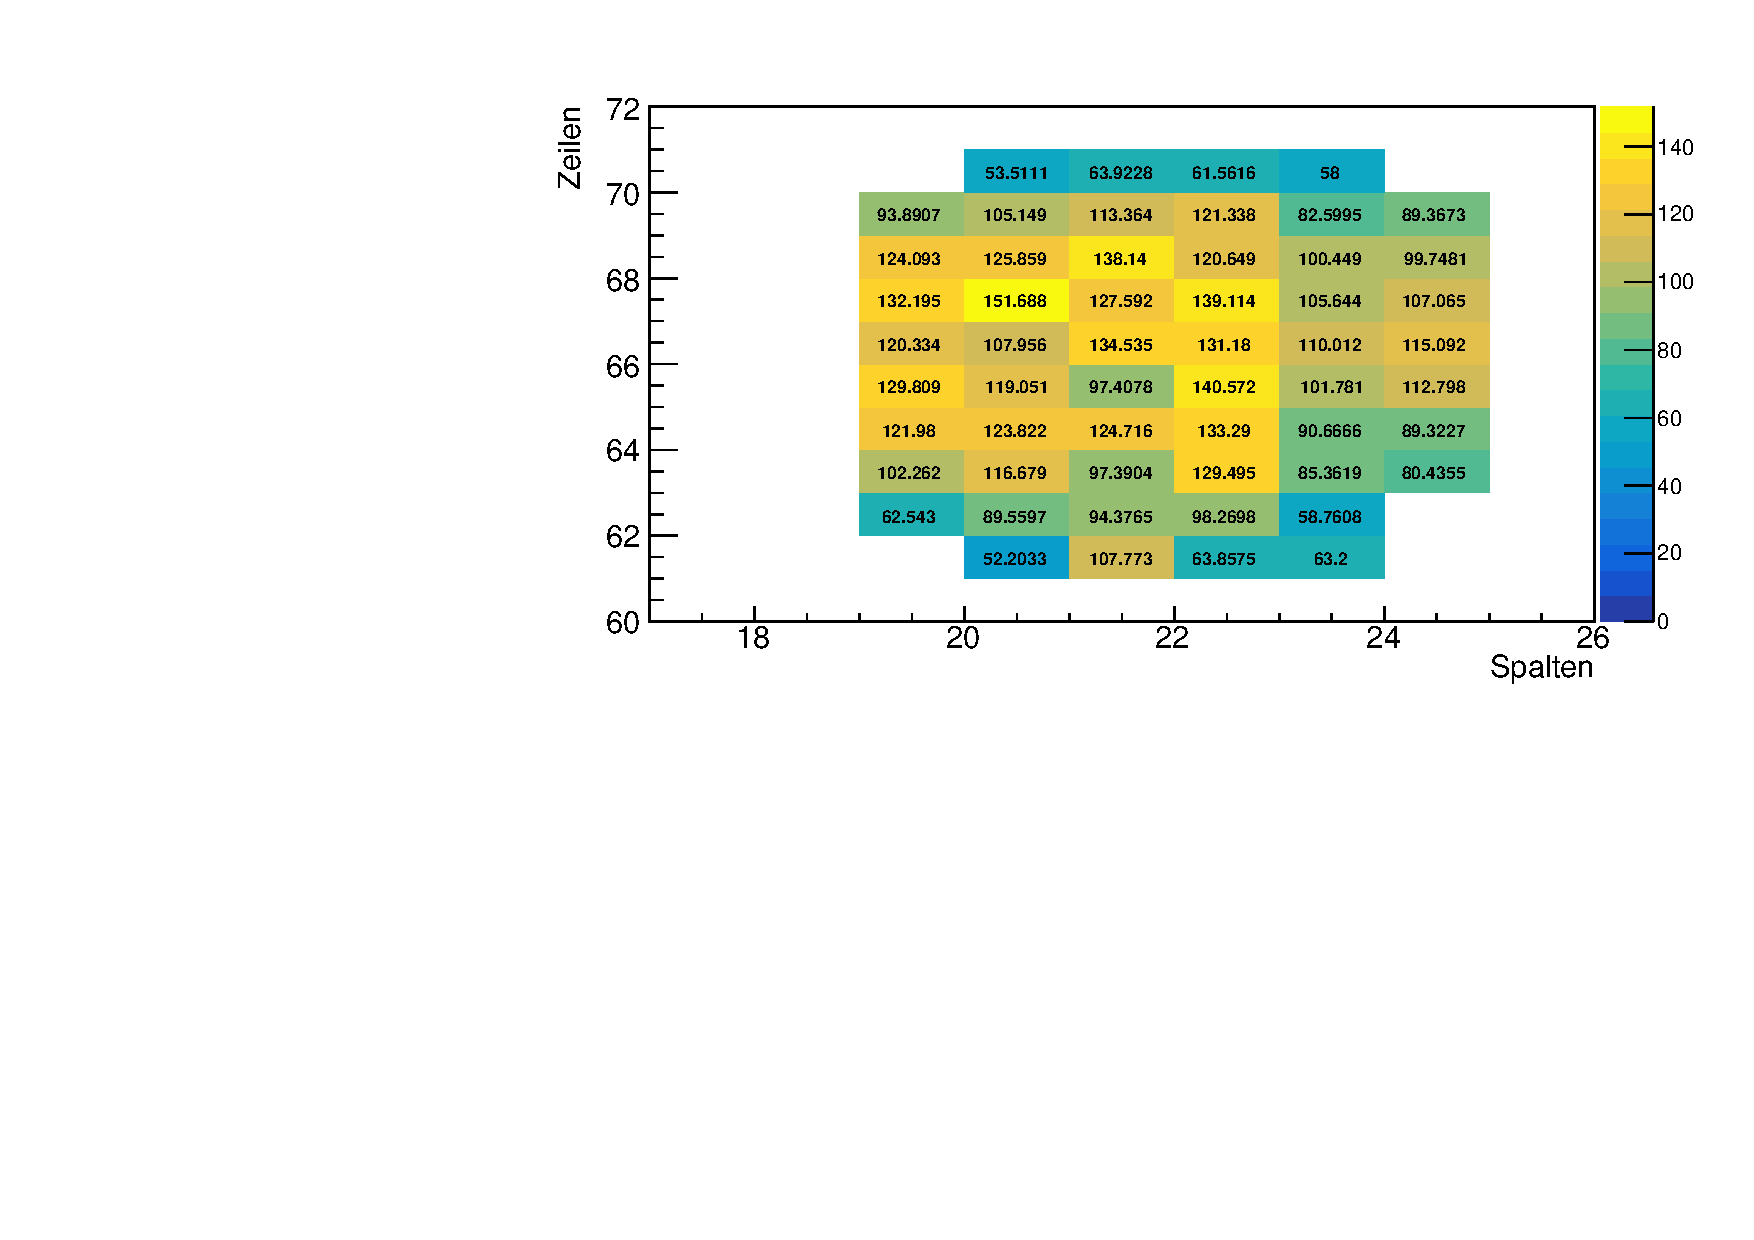
\includegraphics[width=\textwidth]{./15_mm_measurment_plot.pdf}
    \caption{Measured Laserbeam }
    \label{ fig: 5_mm }
  \end{figure}

\end{frame}


\begin{frame}{ Fit - $\SI{15}{\milli\meter}$ }

  \begin{columns}

   \begin{column}{0.48\textwidth}
     \begin{figure}
       \centering
       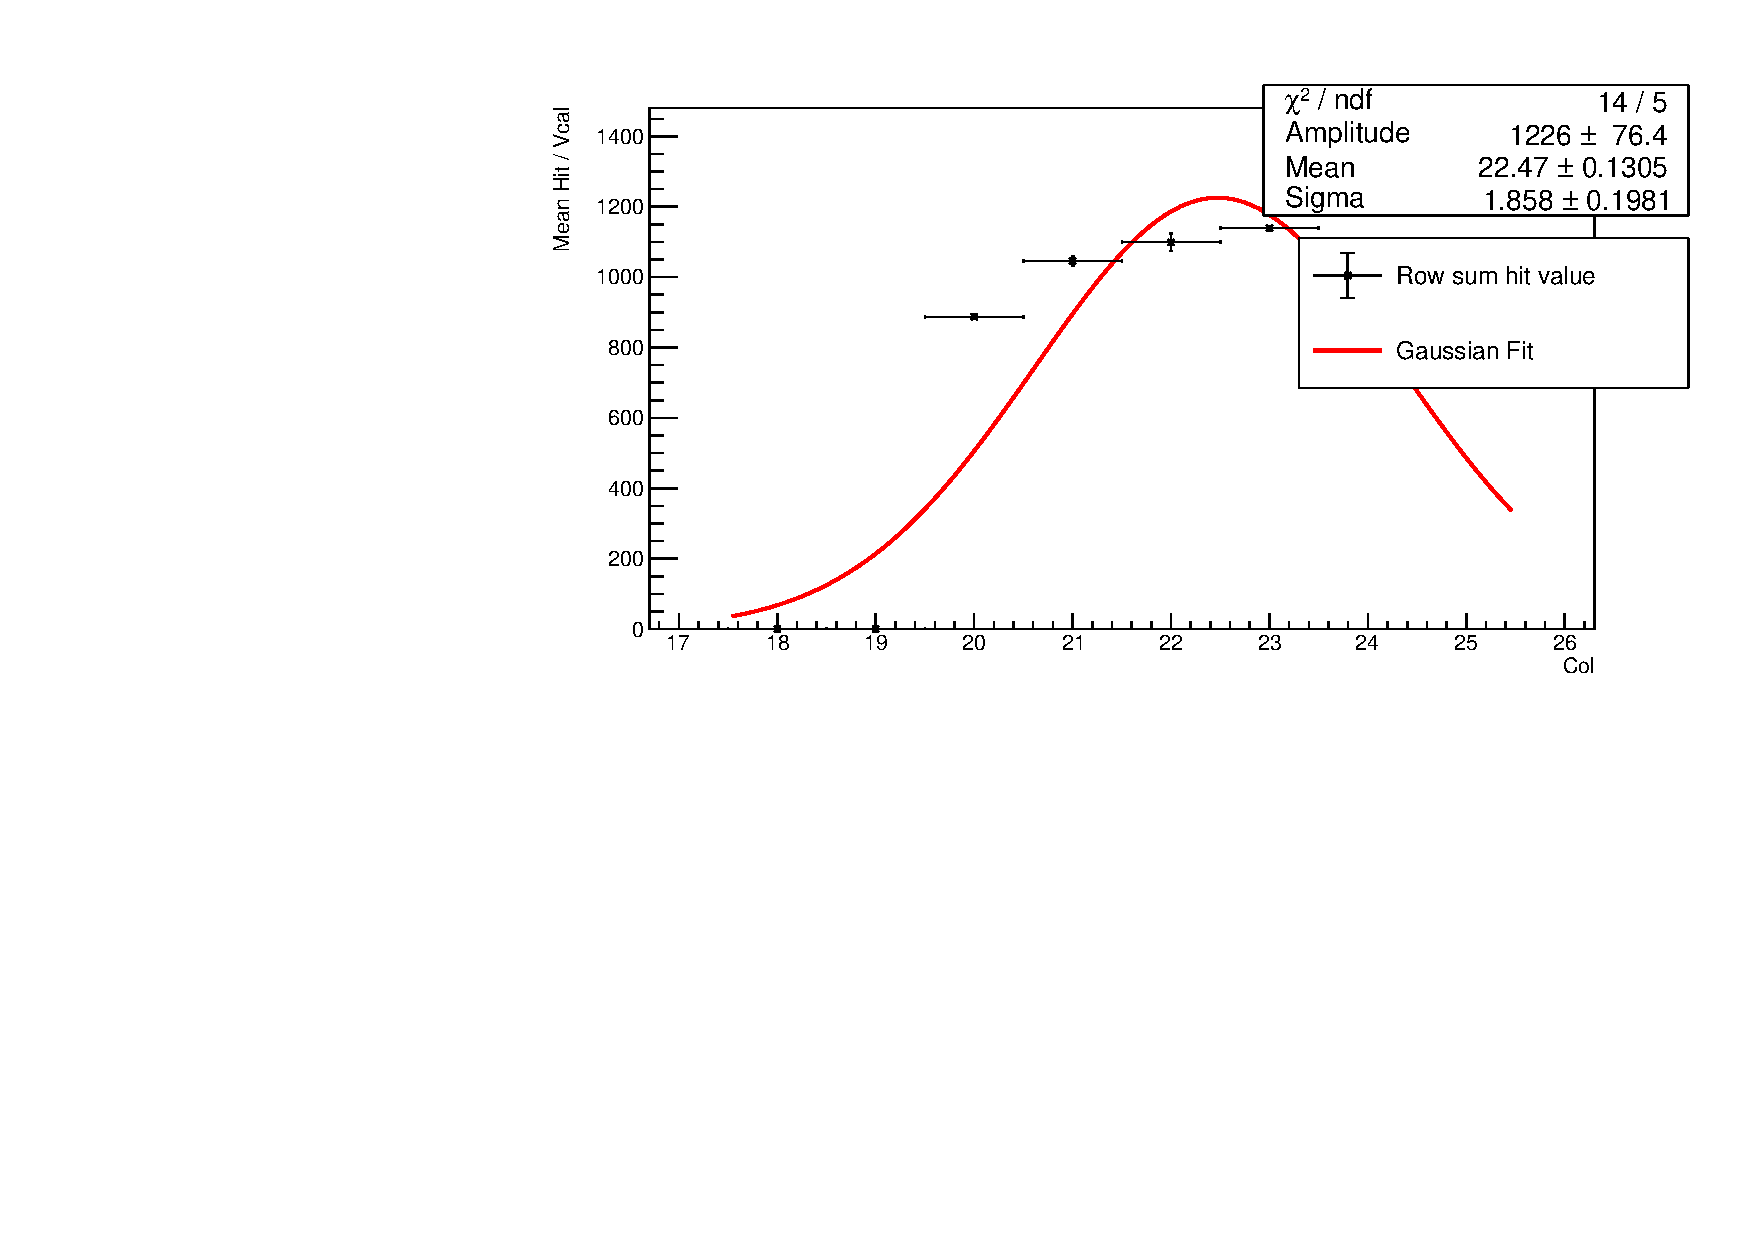
\includegraphics[width=1.05\textwidth]{./15_mm_erorbar_plot_col.pdf}
       \caption{ Fit Columns }
       \label{ fig: iv_curve_theoretical}
     \end{figure}
   \end{column}

   \begin{column}{0.48\textwidth}
     \begin{figure}
       \centering
       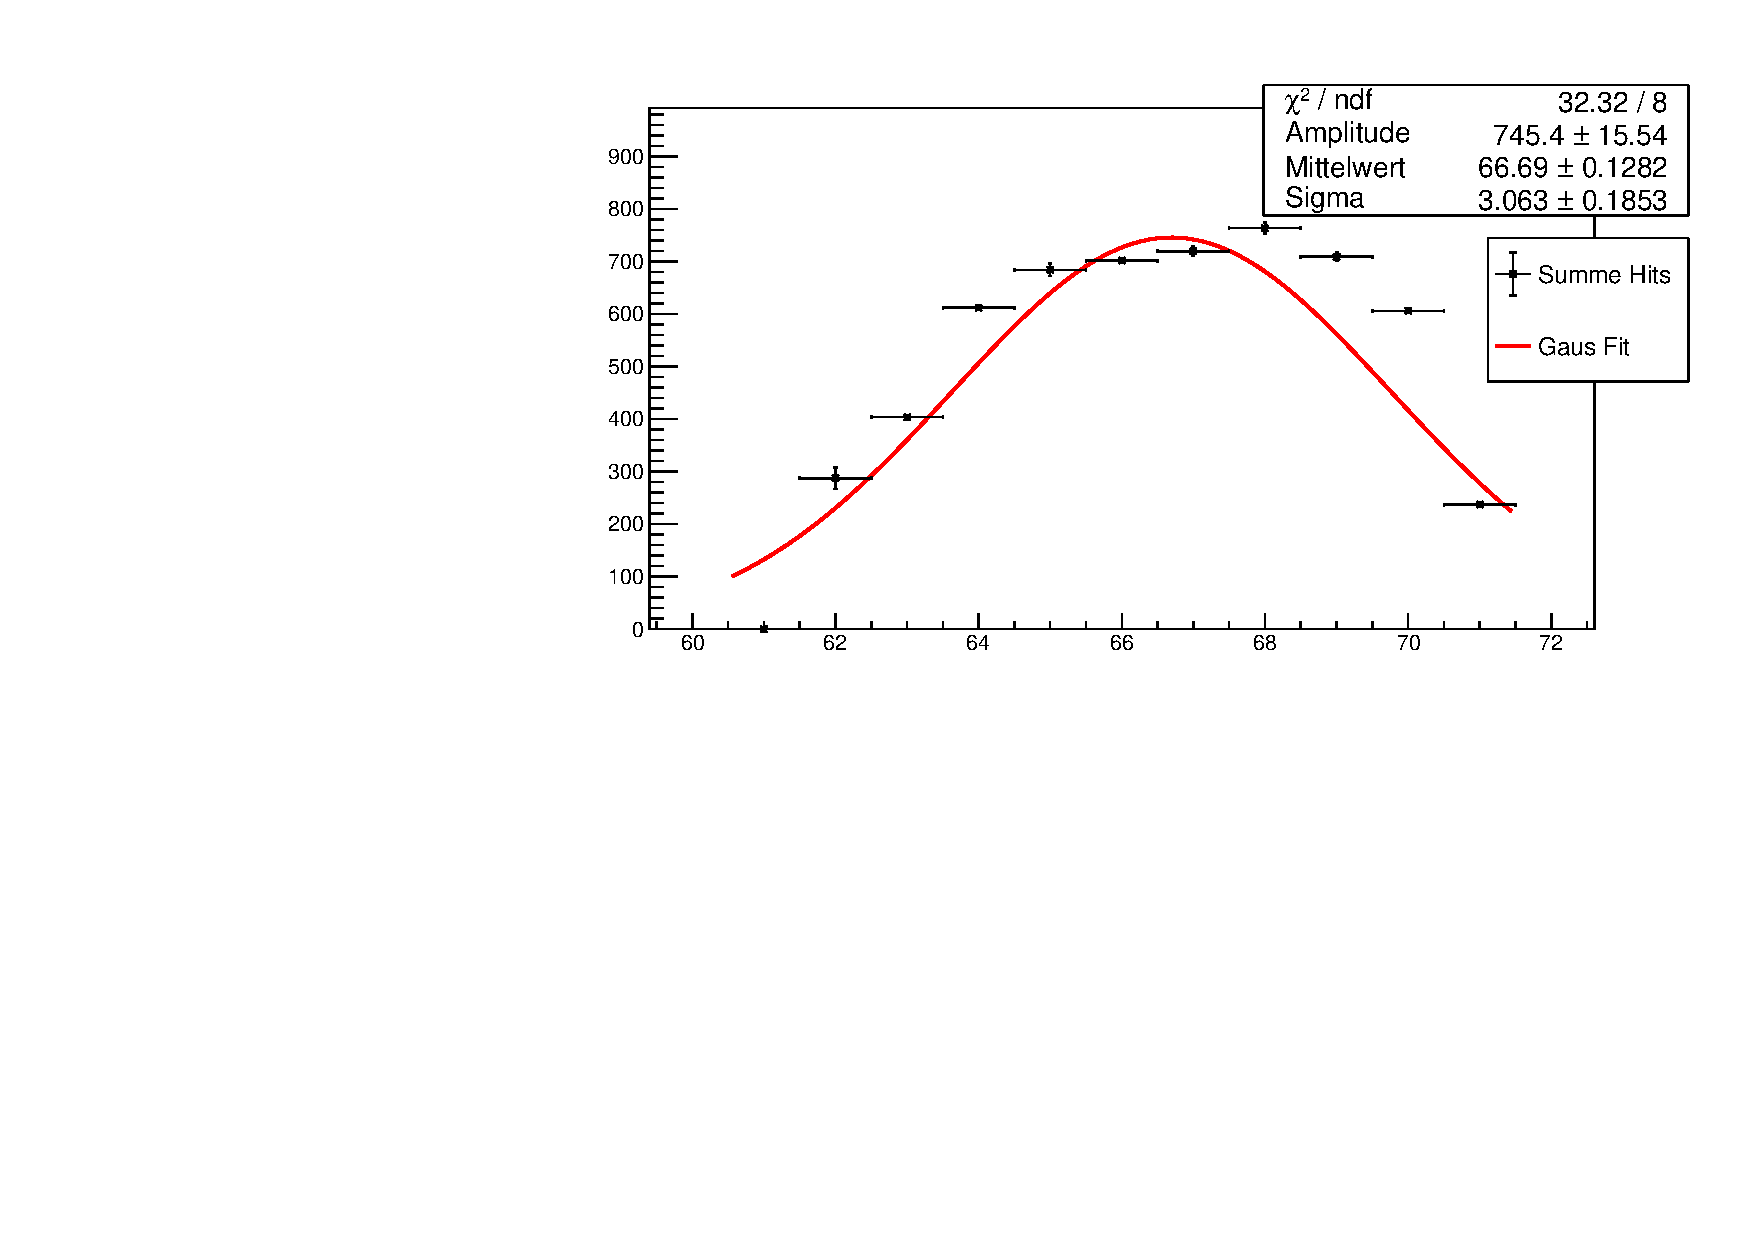
\includegraphics[width=1.05\textwidth]{./15_mm_erorbar_plot_row.pdf}
       \caption{ Fit Rows }
       \label{ fig: iv_curve_measured}
     \end{figure}
   \end{column}

  \end{columns}

\end{frame}

\begin{frame}{ First Result }

     \begin{figure}
       \centering
       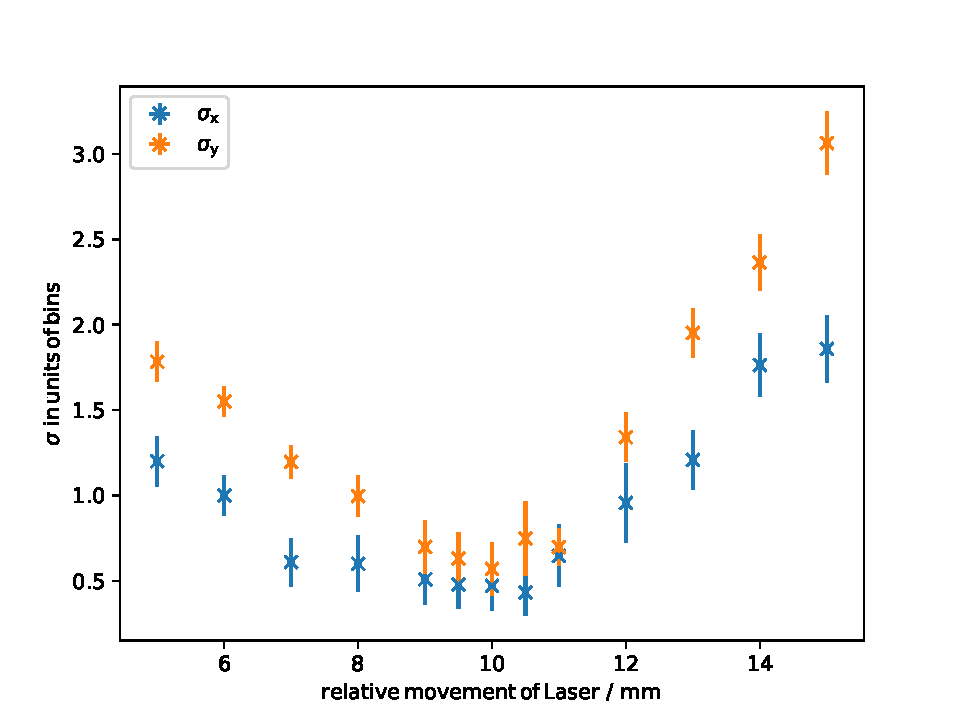
\includegraphics[width=1.05\textwidth]{./perfect_height.pdf}
       \caption{ Sigma against height }
       \label{ fig: iv_curve_theoretical}
     \end{figure}

\end{frame}


\end{document}
